\documentclass[a4paper,kulak]{kulakarticle}

\usepackage[utf8]{inputenc}
\usepackage[dutch]{babel}
\usepackage{pdfpages}
\usepackage{subfig}
\usepackage{float}

\usepackage{cite}

% style
%\usepackage[left=2.5cm,top=2cm,right=2.5cm,bottom=2cm,a4paper]{geometry}
\usepackage{color}

\date{\today}
\address{
	Bachelor in de fysica\\
	Bachelor in de informatica\\
	Bachelor in de wiskunde\\
	Ingenieurswetenschappen}
\title{BDA App}
\author{Marthe B\"{o}ting, Robin Bruneel en Toon Ingelaere}

\begin{document}
	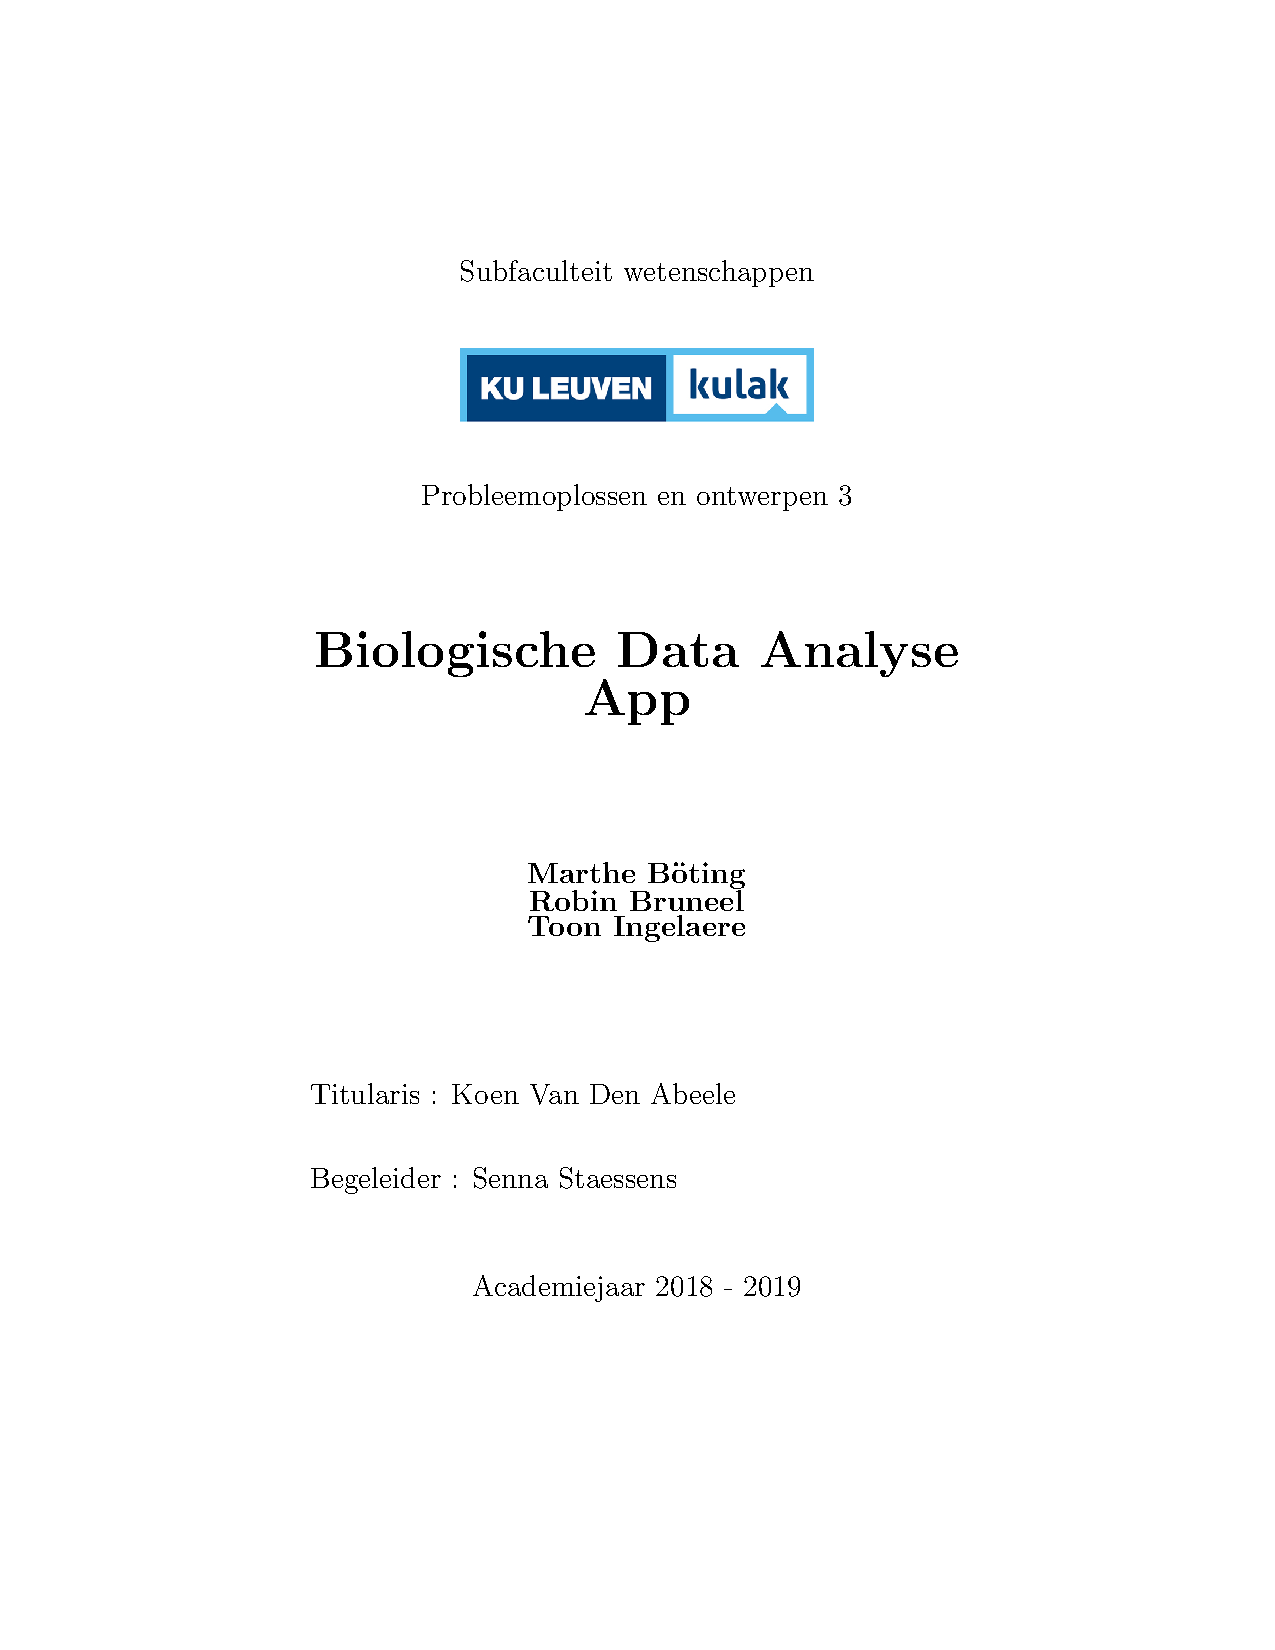
\includepdf{voorblad}
	%\newpage
	
	\maketitle
	\section*{Inleiding}
		

\tableofcontents

\section{Klantenvereisten}


\section{Ontwerpspecificatie}


\section{Onze oplossing}
Dit hoofdstuk is opgedeeld in verschillende deelproblemen: het verwijderen van de achtergrond, het lokaliseren van de indicator en de gebruiksvriendelijke app. Dit alles is gerealiseerd met behulp van de programmeertaal MATLAB.

\subsection{Achtergrondverwijdering}
Het eerste deelprobleem van ons project is het verwijderen van de achtergrond. Op de afbeeldingen is er heel wat vuiligheid te vinden. Voorbeelden hiervan zijn luchtbellen of kleine verkleuringen in de achtergrond zoals men ziet op de Figuur \ref{figuur achtergrondverwijdering}. Hieronder beschrijven we verschillende operaties om de grootste klonters te lokaliseren en alles wat geen klonter is te verwijderen. Dit leidt tot een ruisvrije afbeelding.

\begin{figure}[H]
	\centering
	\includegraphics[width = 0.7\textwidth]{Ruis_afbeelding.png}	
	\caption{In de rechterbovenhoek zien we luchtbellen en in de onderste cirkel zien we een verkleuring die geen deel uitmaakt van een bloedklonter.}
	\label{figuur achtergrondverwijdering}
\end{figure}

\subsubsection{Bepalen van de beste threshold}
Het onderscheid tussen de achtergrond (eerder wit) en de bloedklonter (eerder grijs) is makkelijker te zien op de grijswaarden van de afbeelding, zie Figuur \ref{figuur beste_threshold}.. Daarnaast is één grijswaarde voldoende om het onderscheid te maken. Wanneer een histogram opgesteld wordt van deze waarden is een duidelijk dipje tussen het wit en het grijs te zien, zie Figuur \ref{figuur graf1}. Dit is dan ook de theoretisch optimale threshold, de grijswaarde om een bloedklonterpixel van een achtergrondpixel te onderscheiden. Deze bepalen we simpelweg als het minimum in de tweede helft van de histogram. Na het toepassen van de threshold komt de binaire Figuur \ref{figuur foto_bin} tevoorschijn. Dit lijkt de klonters nagenoeg goed te detecteren.

\begin{figure}[H]
	\centering
	\subfloat[]{{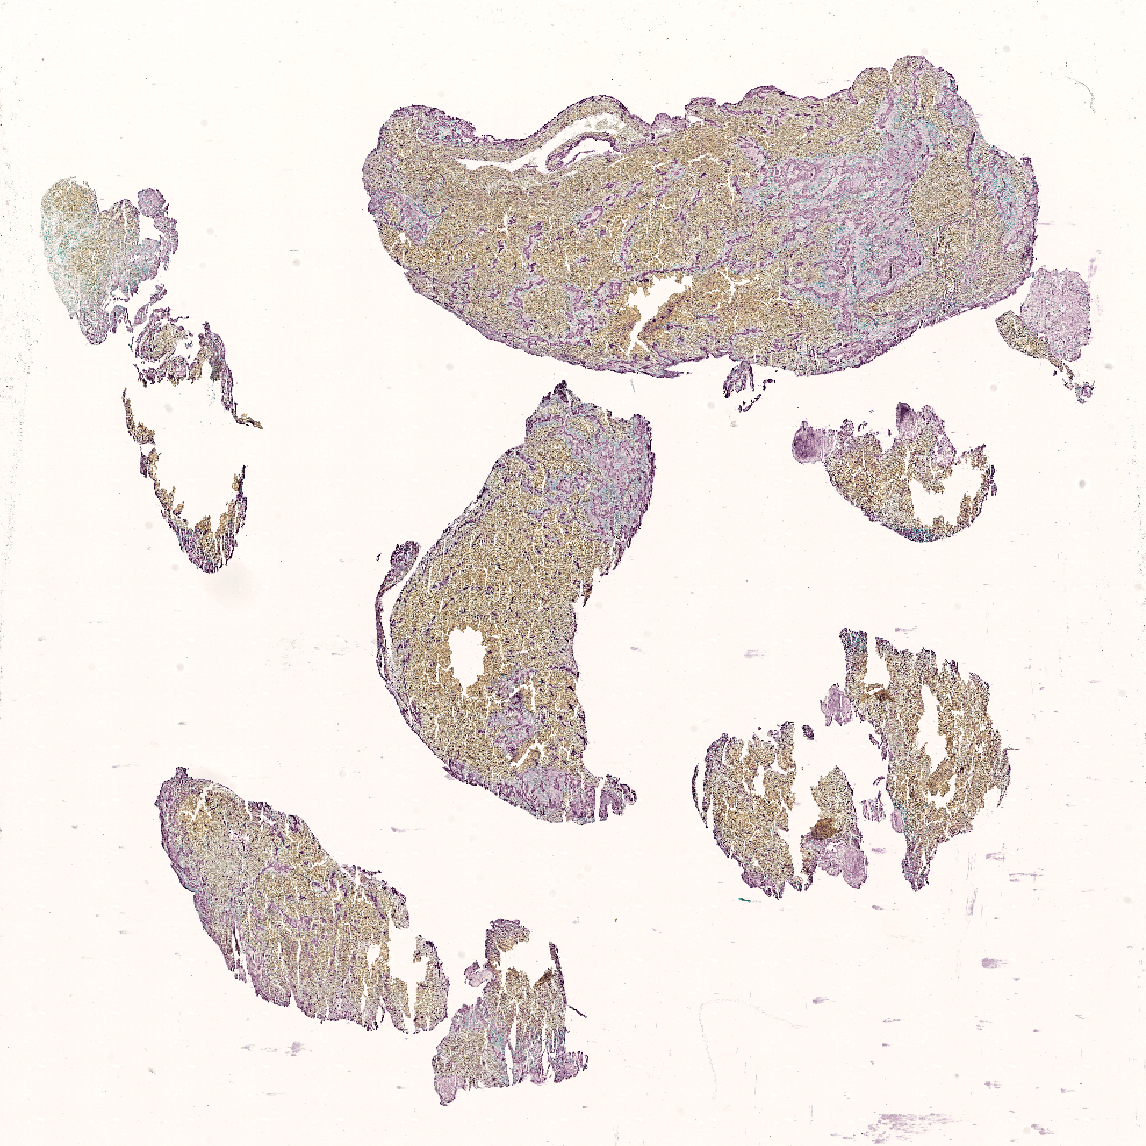
\includegraphics[width=6cm]{origineel_vb}}}
	\qquad
	\subfloat[]{{\includegraphics[width=6cm]{grijswaarden_vb}}}
	
	\caption{Illustratie van de originele foto (a) en deze omgezet in grijswaarden (b).}
	\label{figuur beste_threshold}
\end{figure}

\begin{figure}[H]
	\centering
	\includegraphics[width=0.85\textwidth]{GetBestthreshold_vb_aangeduid.png}
	
	\caption{Histogram van het aantal pixels gegroepeerd per grijswaarde. We zien duidelijk een lokaal minimum rond de waarde 230. Opmerking: we maken hier gebruik van een logaritmische y-as.}
	\label{figuur graf1}
\end{figure}

\begin{figure}[H]
	\centering
	\includegraphics[width=0.7\textwidth]{grijswaarden_bin_vb}
	\caption{Op deze binaire representatie zijn de bloedklonters duidelijk te zien.}
	\label{figuur foto_bin}
\end{figure}

\subsubsection{Ruisfilter}
Eenmaal de binaire representatie is opgesteld, kunnen de bloedklonters nauwkeurig gelokaliseerd worden door al het overbodige ruis te verwijderen. De ruis kan makkelijk verwijderd worden door alle kleine groepen witte/zwarte pixels respectievelijk te vervangen door zwarte/witte pixels. Het resultaat is te zien op Figuur \ref{figuur ruisfilter} (a). \\
Deze zogenaamde 'mask'\footnote{Bij het toepassen van een mask op een afbeelding, worden alle pixels in de afbeelding die zwart zijn in de mask, wit gemaakt. De andere pixels behouden hun kleur.} kan toegepast worden op de originele afbeelding om de ruisvrije afbeelding te vormen. Daarnaast wordt deze afbeelding bijgesneden om kostbare geheugenruimte te sparen, zoals te zien is in Figuur \ref{figuur ruisfilter} (b). In dit deelprobleem werd echter met een reeds bijgesneden bloedklonter gewerkt om de afbeeldingen duidelijk te houden. Een volledig onbewerkte afbeelding is echter te zien in Figuur \ref{figuur volledig_onbewerkt}

\begin{figure}[H]
	\centering
	\subfloat[]{{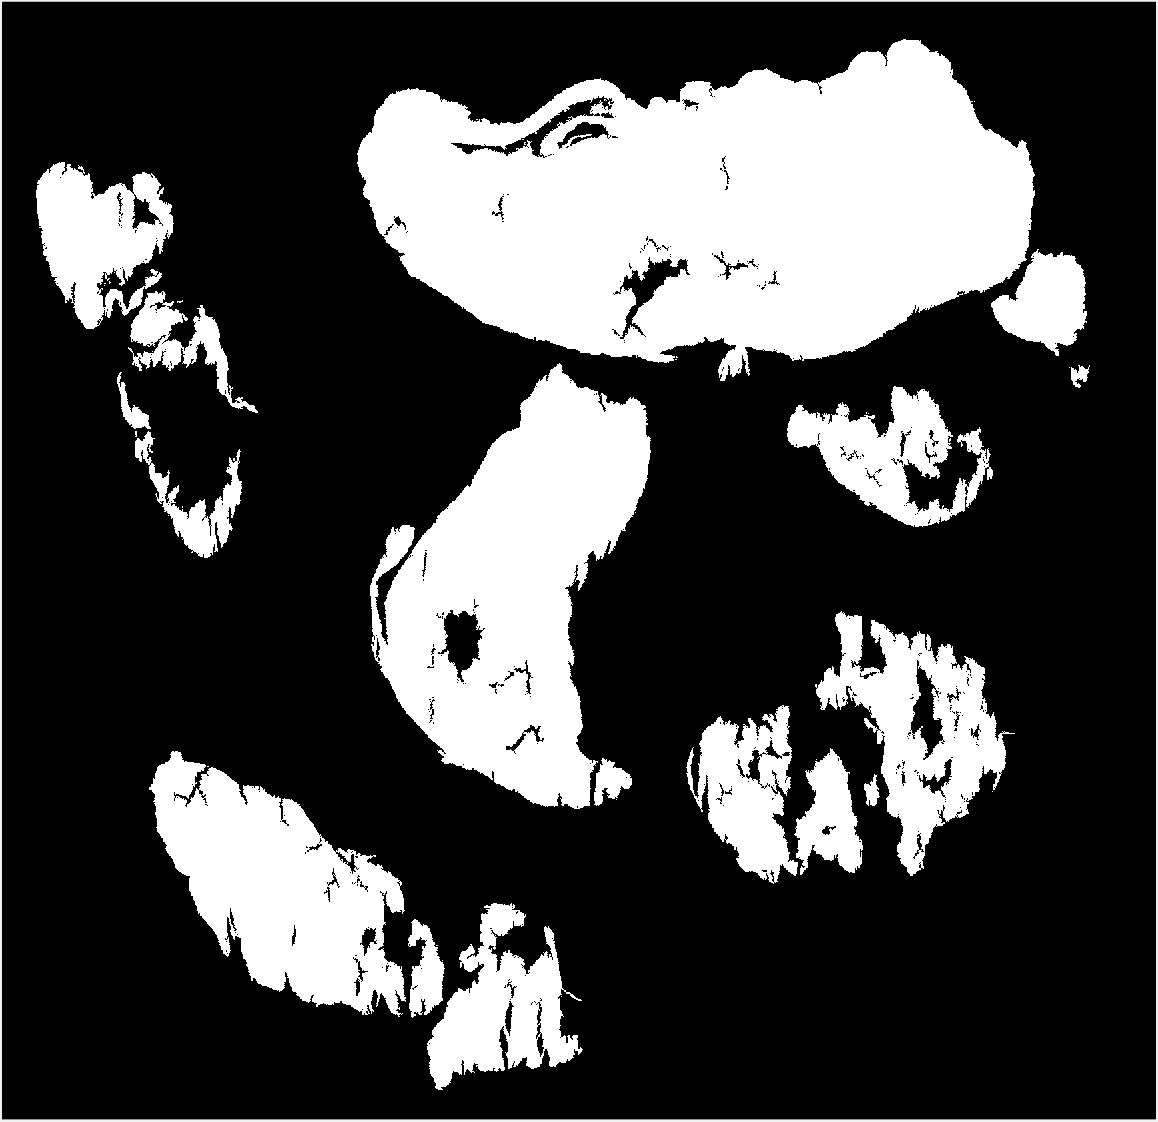
\includegraphics[width=7cm]{ruisvrij_vb}}}
	\qquad
	\subfloat[]{{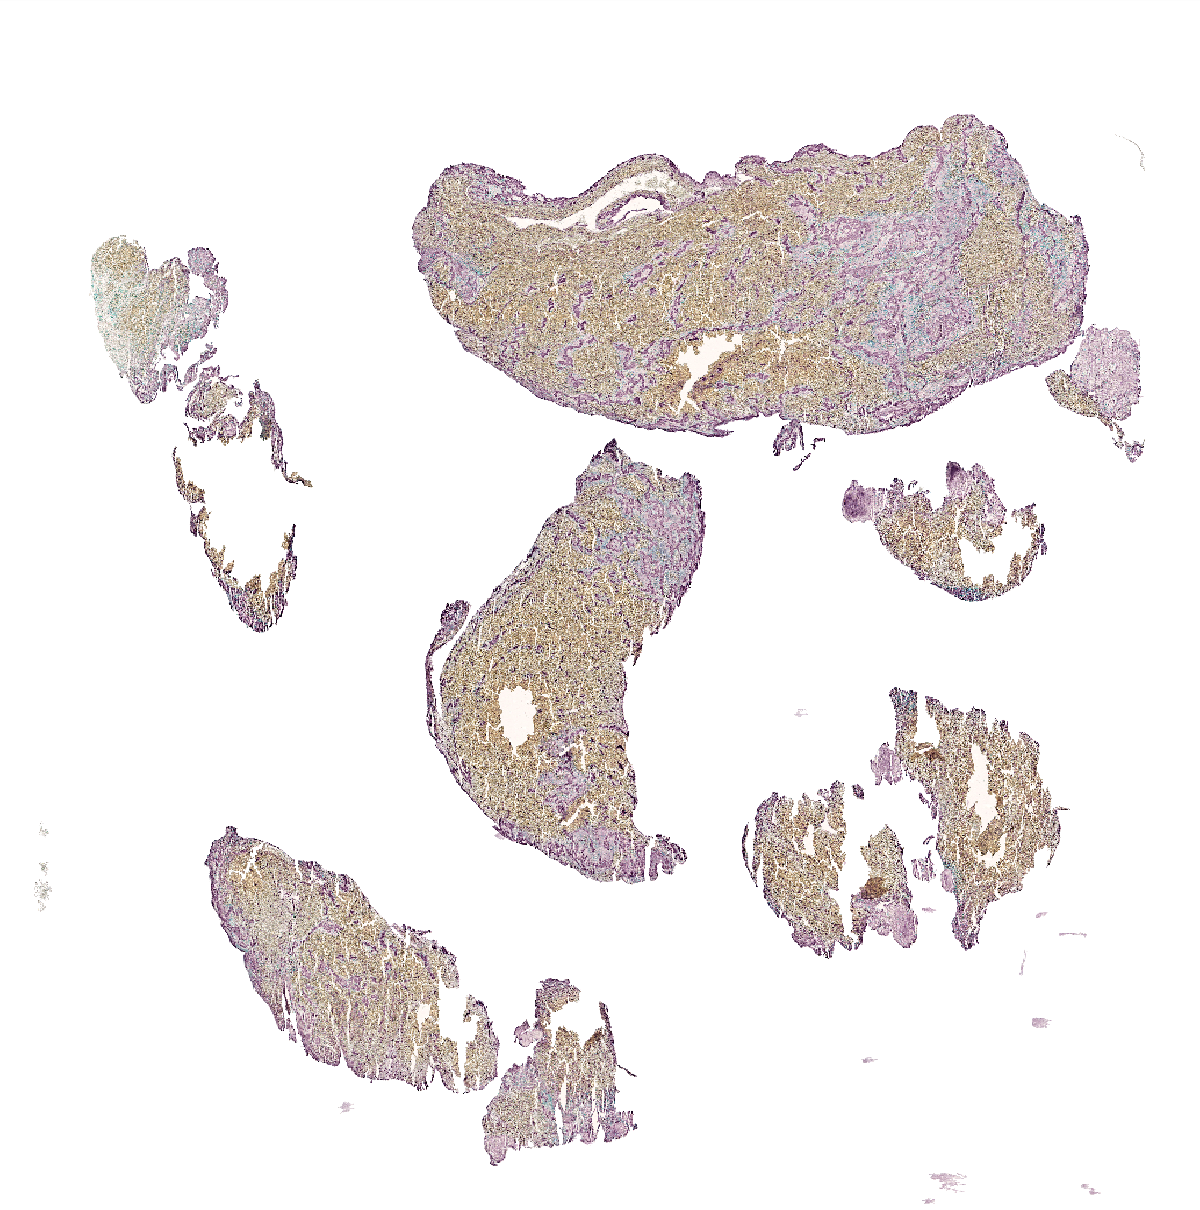
\includegraphics[width=7cm]{ruisvrij_kleur_vb}}}
	
	\caption{Alle ruis is verwijderd, dit is een foto waarmee we kunnen werken.}
	\label{figuur ruisfilter}
\end{figure}

\begin{figure}[H]
	\centering
	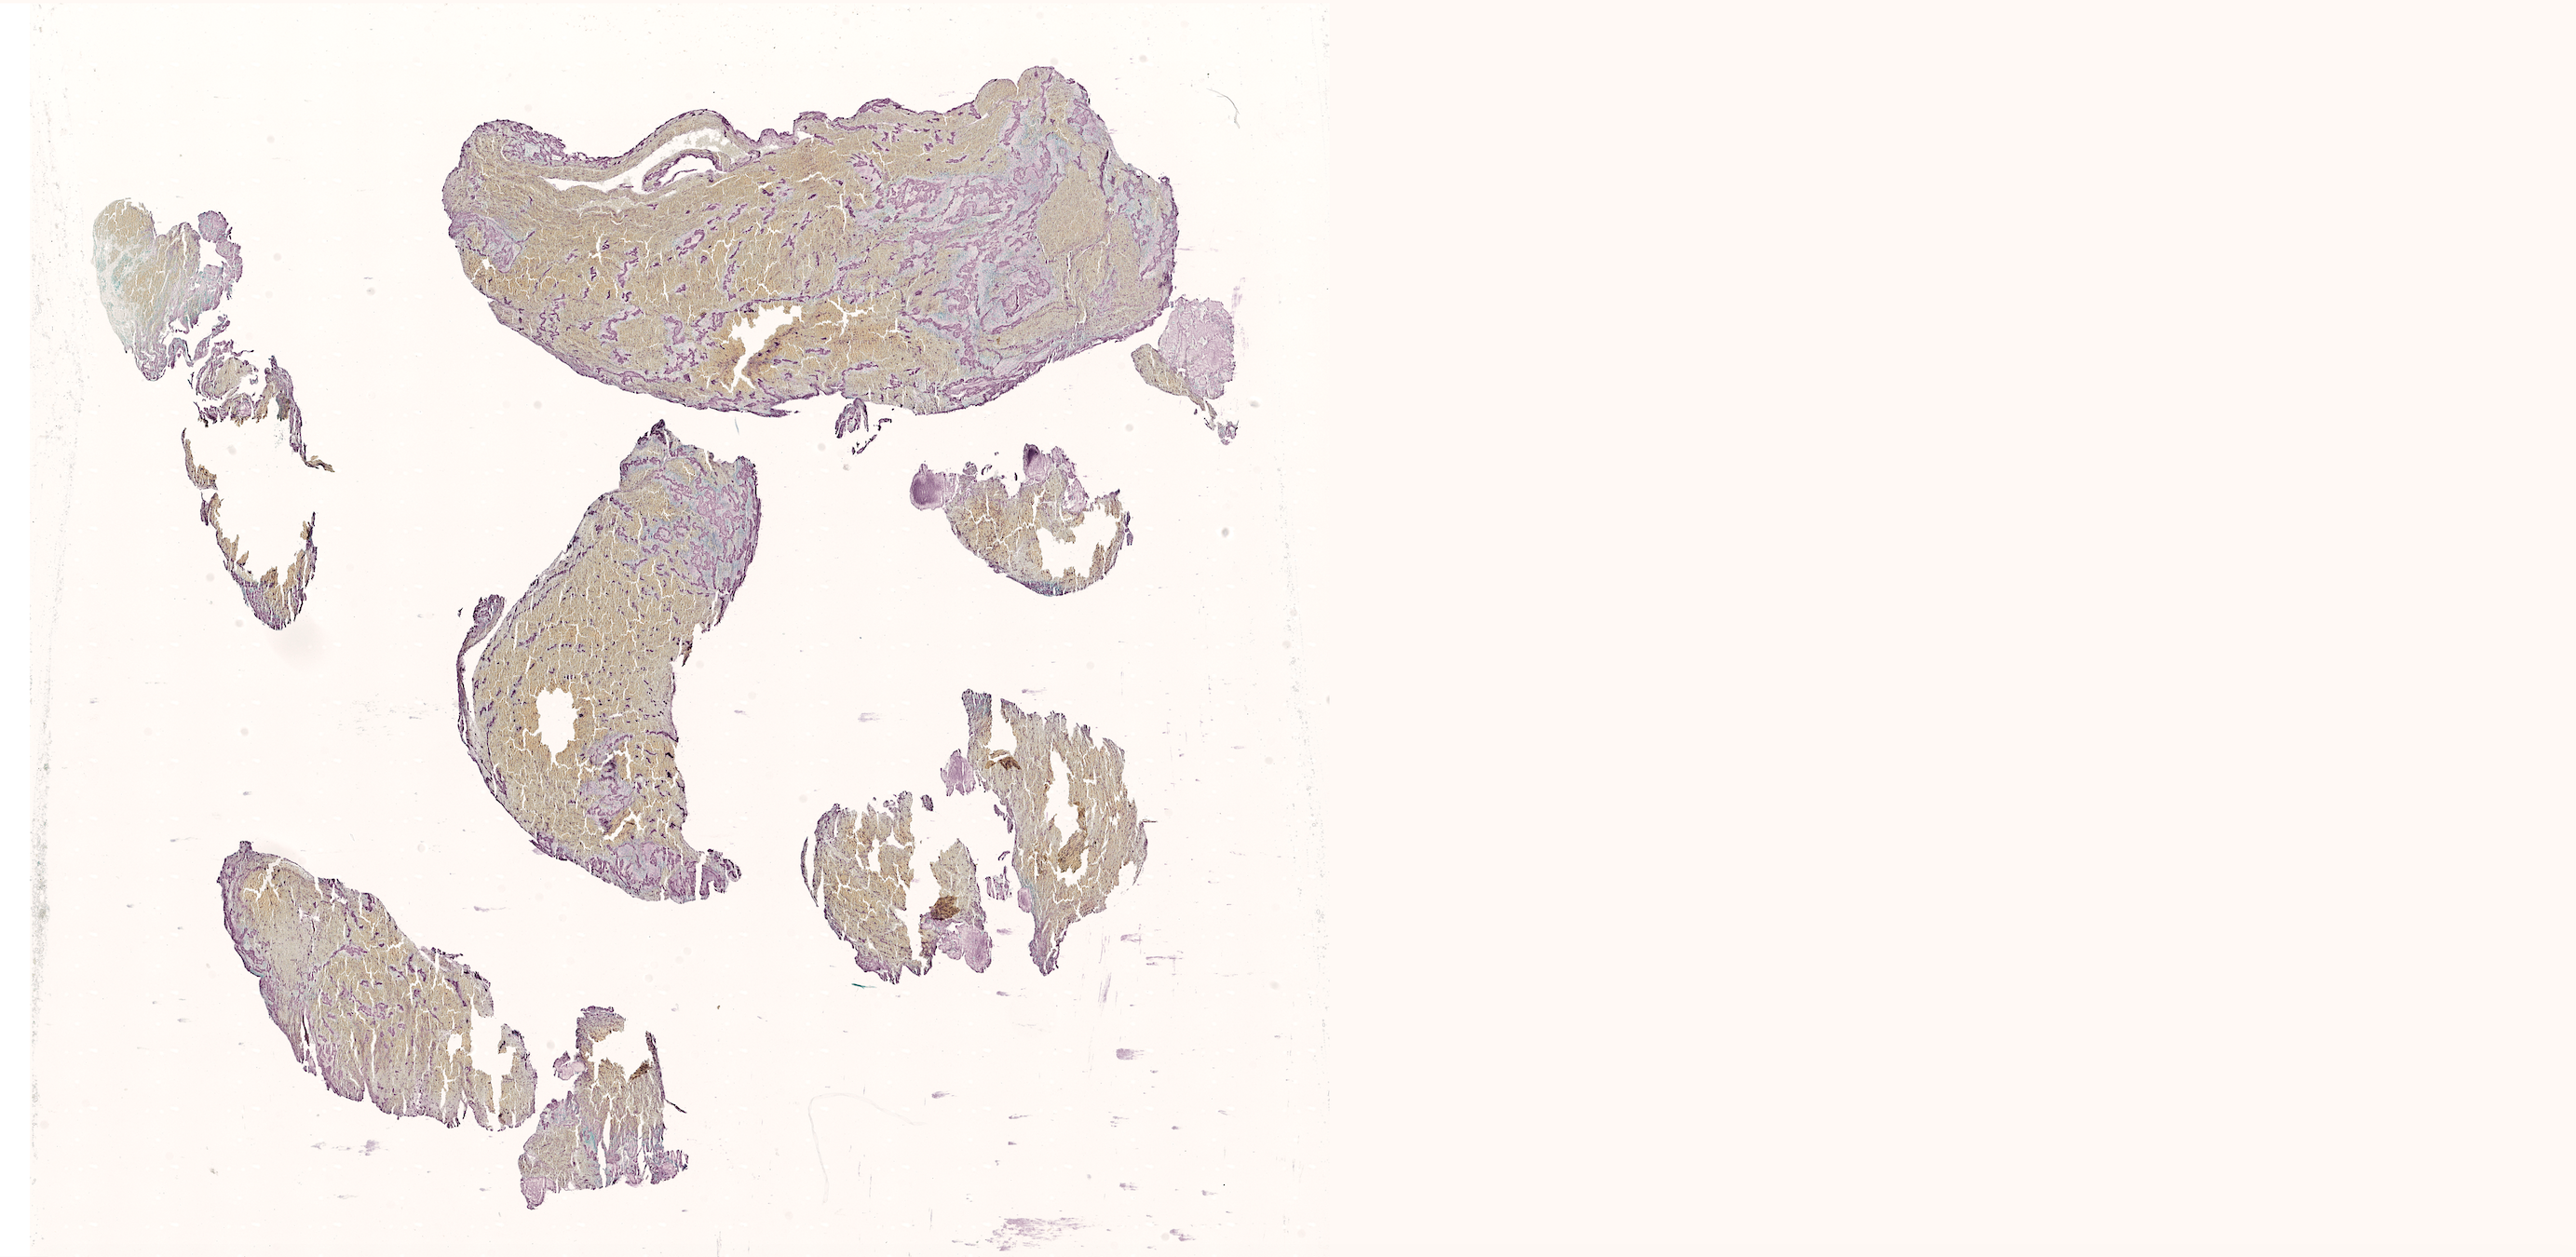
\includegraphics[width=15.25cm]{Volledig_onbewerkt}
	
	\caption{Dit is een volledig onbewerkte afbeelding die we in \ref{figuur ruisfilter} (b) hebben bijgesneden en waarvan de achtergrond verwijderd is.}
	\label{figuur volledig_onbewerkt}
\end{figure}
\subsection{Lokalisatie van de indicator}
Het tweede deel van ons project is de indicators lokaliseren en kwantificeren. We hebben de opdracht gekregen twee soorten te kunnen onderscheiden. Van deze is een voorbeeld op Figuur \ref{figuur indicators} te zien. Omdat het kleurverschil tussen indicator en achtergrond niet altijd even groot is, vormen we het oorspronkelijke \textit{RGB} kleurmodel\footnote{Het RGB kleurmodel is een voorstelling waarbij ieder kleur voorgesteld wordt door een waarde van de drie basiskleuren (rood, groen en blauw)} om naar het zogenaamde \textit{HSV} kleurmodel. Dit model is een alternatieve voorstelling waarbij men alle kleuren op een cirkel voorstelt, de hoek die dit kleur dan maakt, noemt men de \textit{Hue}. Naast deze waarde heeft \textit{HSV} nog twee andere parameters namelijk \textit{Saturation} en \textit{Value}. \textit{Saturation} kan simpel beschouwd worden als een aanduiding van de hoeveelheid witte kleur en \textit{Value} een aanduiding van de zwarte kleur. Een grafische voorstelling is te zien op Figuur \ref{figuur hsv_schema}.\\
Het voordeel van deze transformatie is dat het heel wat eenvoudiger is om een onderscheid tussen dichtbijgelegen kleuren te vinden. Een andere mogelijke transformatie is die naar het \textit{LAB} of het \textit{CMYK} kleurmodel die gelijkaardige eigenschappen heeft en desnoods ook gebruikt kan worden. Eenmaal we een duidelijk onderscheid tussen de indicator en de achtergrond maken, kunnen we eenvoudig het percentage indicator berekenen door het aantal bloedklonter- en indicatorpixels op te tellen. Ons stappenplan wordt in volgende hoofdstukken besproken en wordt toegepast op de afbeelding uit Figuur \ref{figuur indicators} (a).

\begin{figure}[H]
	\centering
	\subfloat[]{{\includegraphics[width=7cm]{Indicator_vb1}}}
	\qquad
	\subfloat[]{{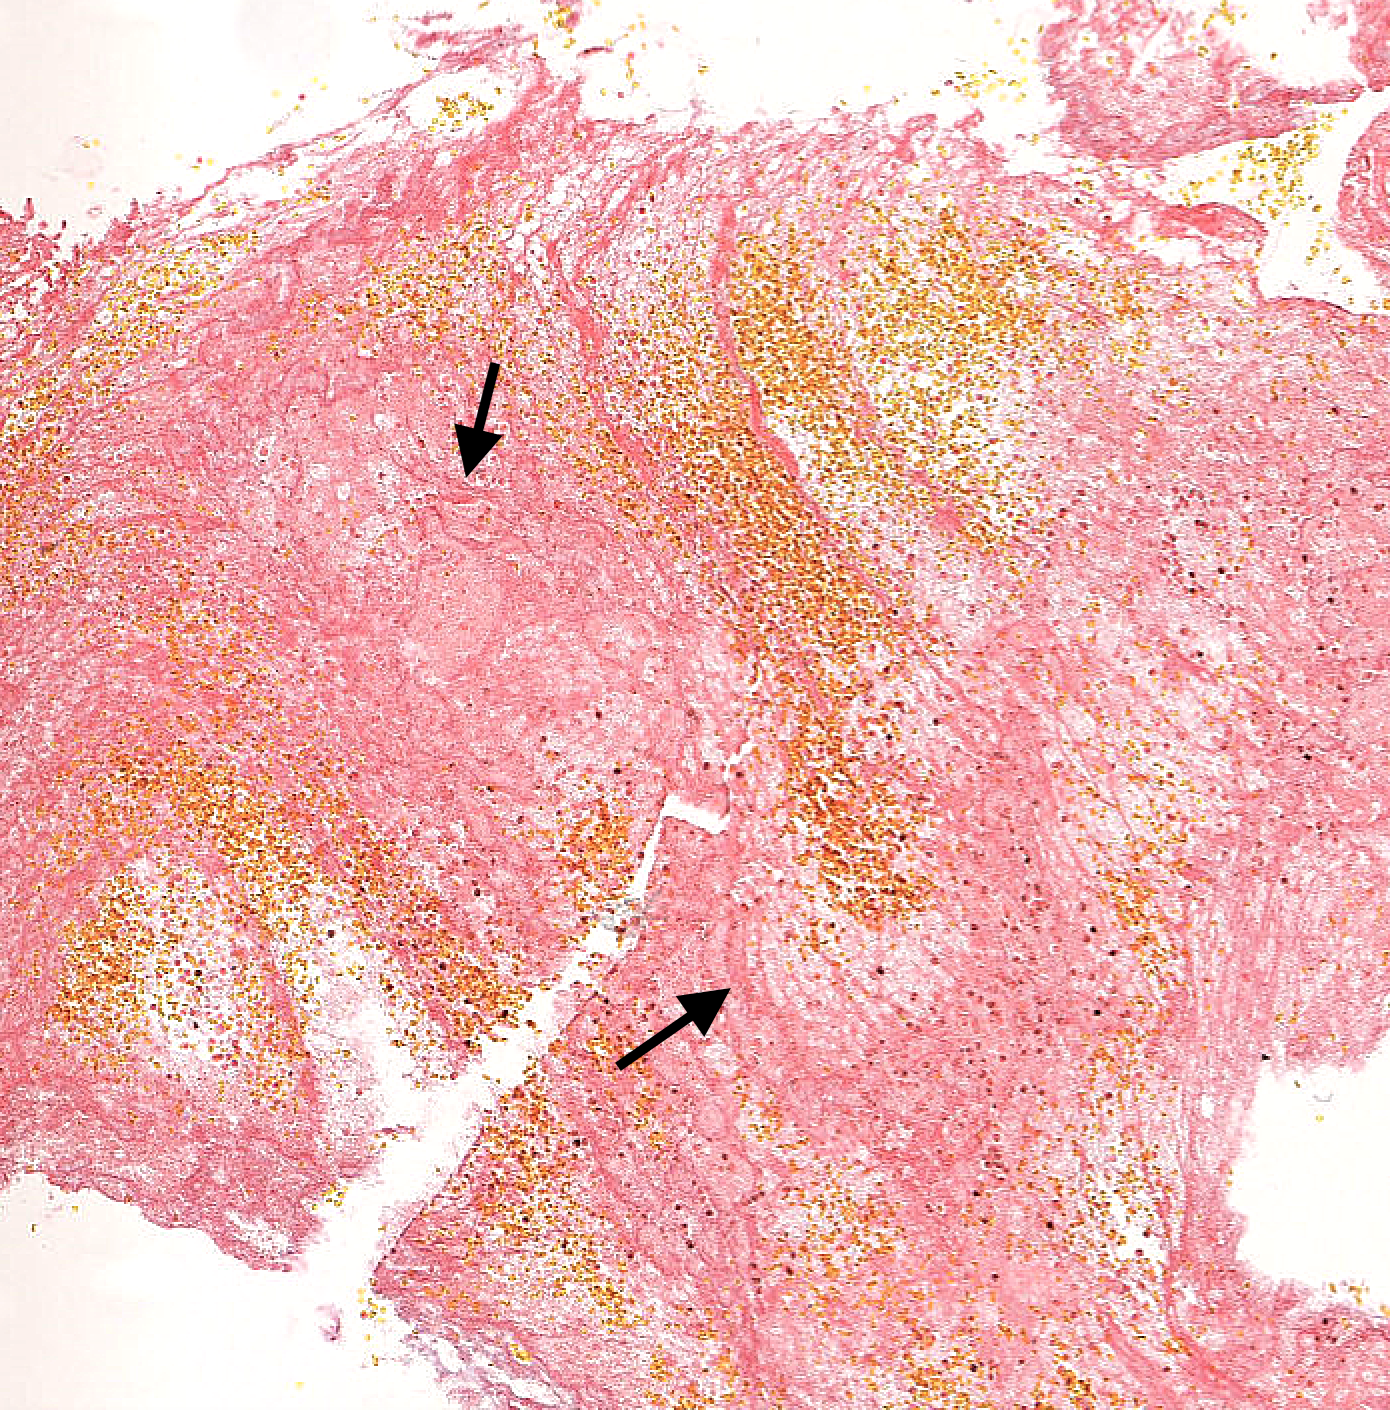
\includegraphics[width=7cm]{Indicator_vb2}}}
	
	\caption{Illustratie van de twee soorten indicator (respectievelijk paars en donkerroze) die gedetecteerd moeten worden. We zien duidelijk dat het detecteren op afbeelding (a) eenvoudiger zal zijn dan op afbeelding (b).}
	\label{figuur indicators}
\end{figure}

\begin{figure}[H]
	\centering
	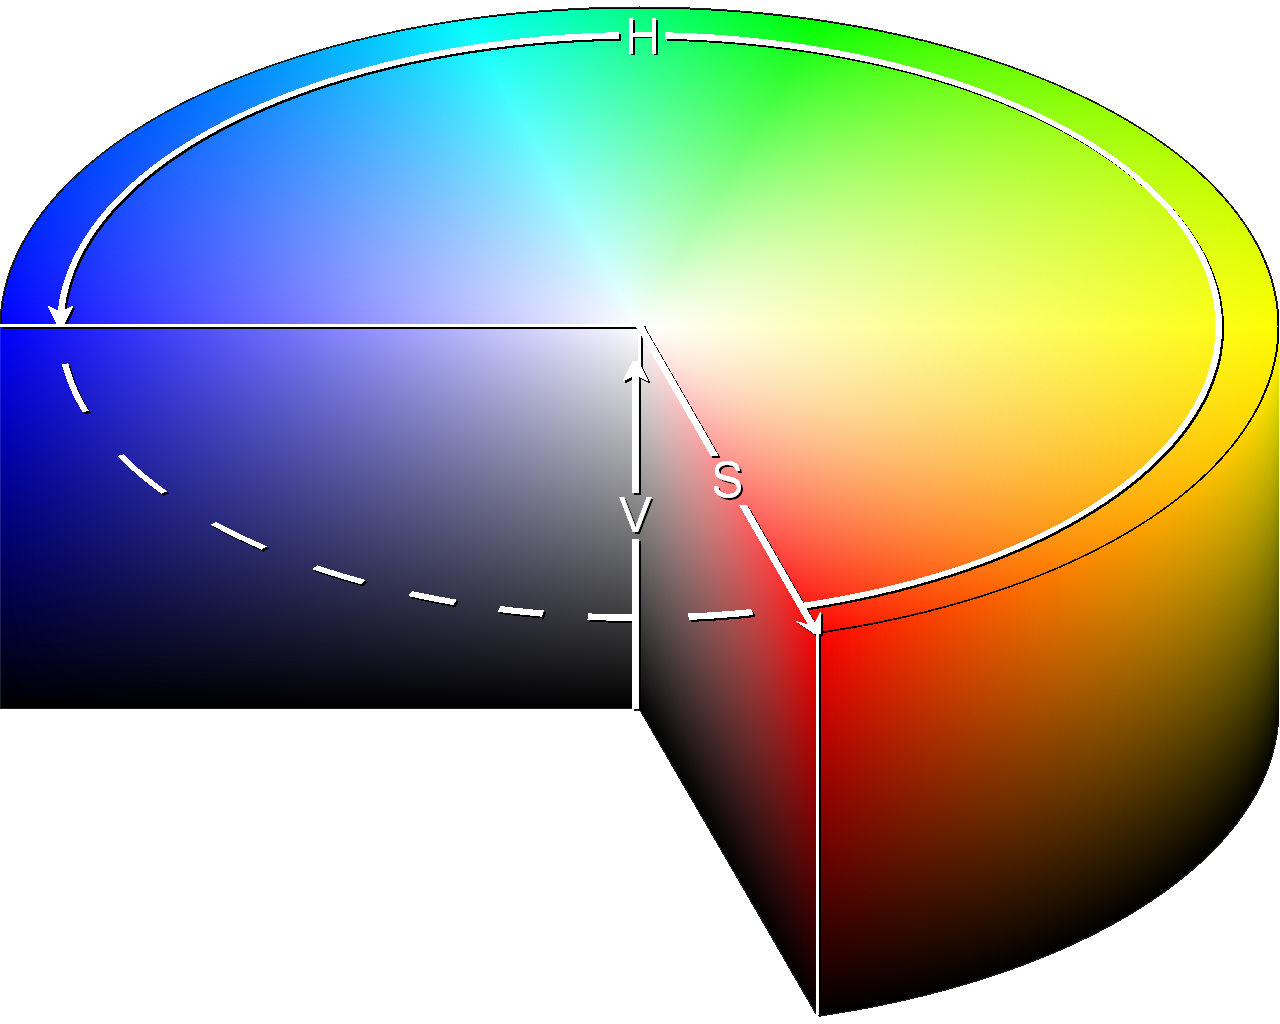
\includegraphics[width=0.7\textwidth]{HSV_vb.png}
	
	\caption{Grafische voorstelling van het \textit{HSV} (\textit{Hue}, \textit{Saturation}, \textit{Value}) kleurmodel}
	\label{figuur hsv_schema}
\end{figure}

\subsubsection{Het HSV kleurmodel}
Zoals reeds vermeld, beginnen we met een transformatie naar het \textit{HSV} kleurmodel. Bijgevolg kunnen we de twee voorstellingen vergelijken. We hebben het model telkens ontbonden in de drie kleurwaarden, waarbij zwart de laagste waarde voor dat kleur is en wit de hoogste. De resultaten zijn te zien in de Figuren \ref{figuur RGB} en \ref{figuur HSV}. Het verschil tussen de twee kleurmodellen is duidelijk te zien. Afbeelding (a) en (b) uit Figuur \ref{figuur HSV} lijken namelijk een iets agressiever onderscheid te maken.

\begin{figure}[H]
	\centering
	\subfloat[]{{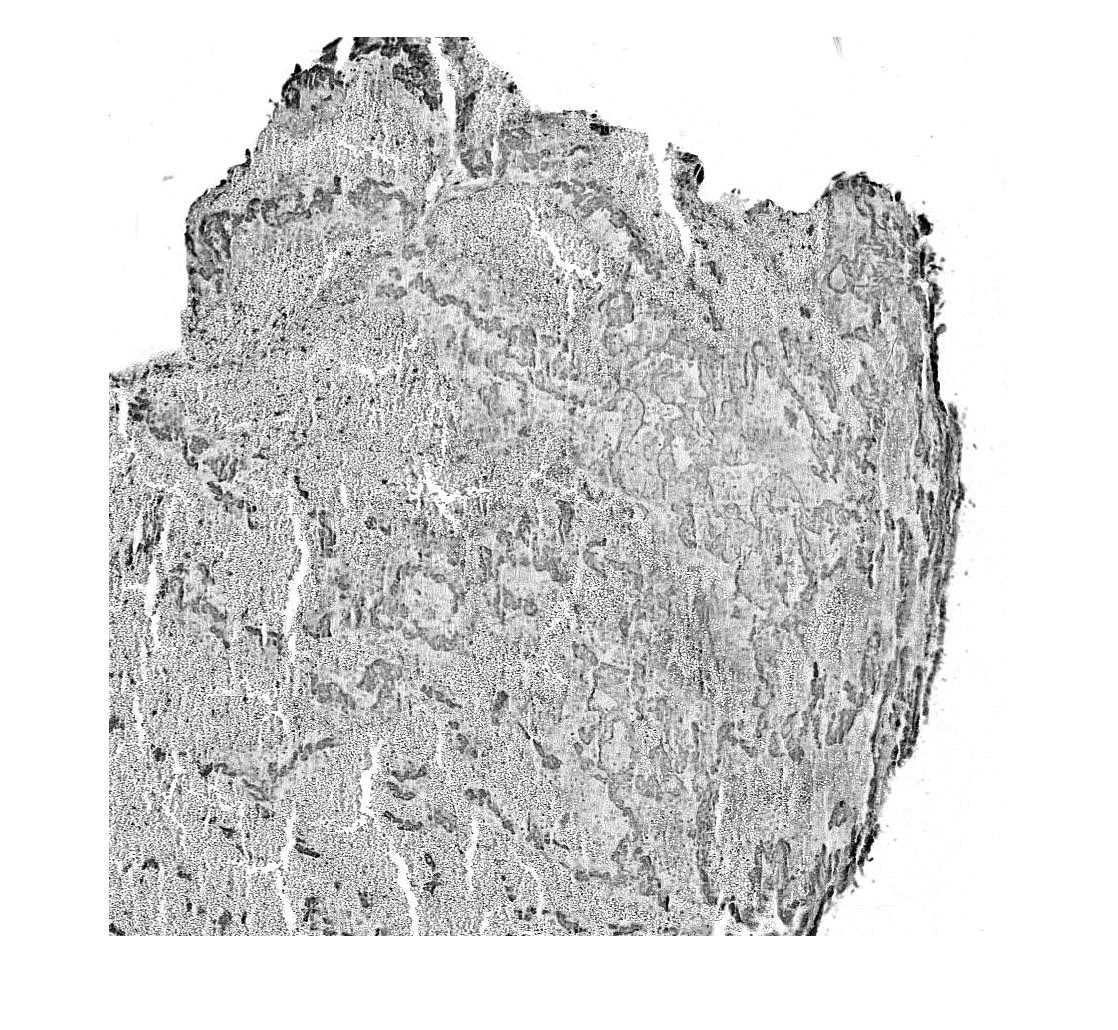
\includegraphics[width=4.5cm]{RGB_r}}}
	\qquad
	\subfloat[]{{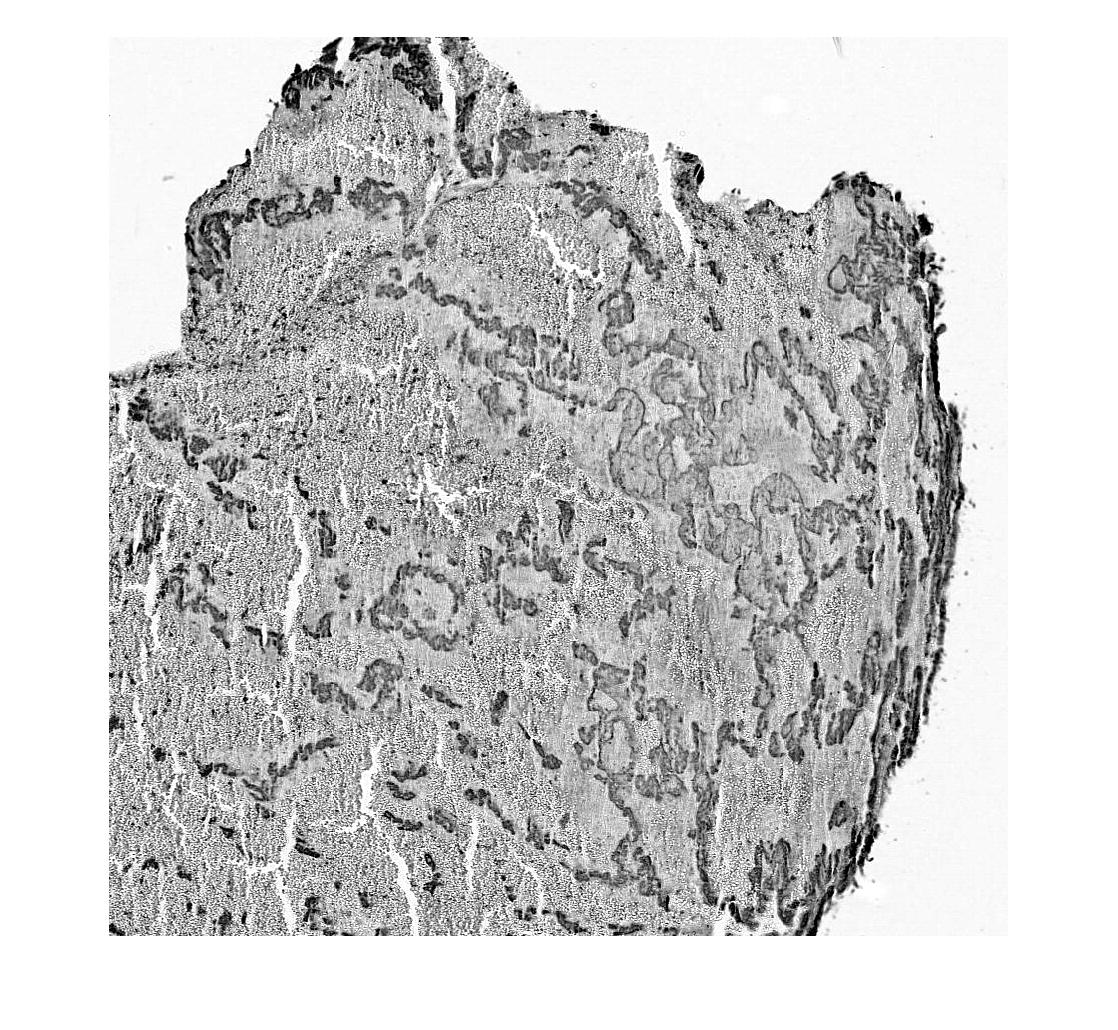
\includegraphics[width=4.5cm]{RGB_g}}}
	\qquad
	\subfloat[]{{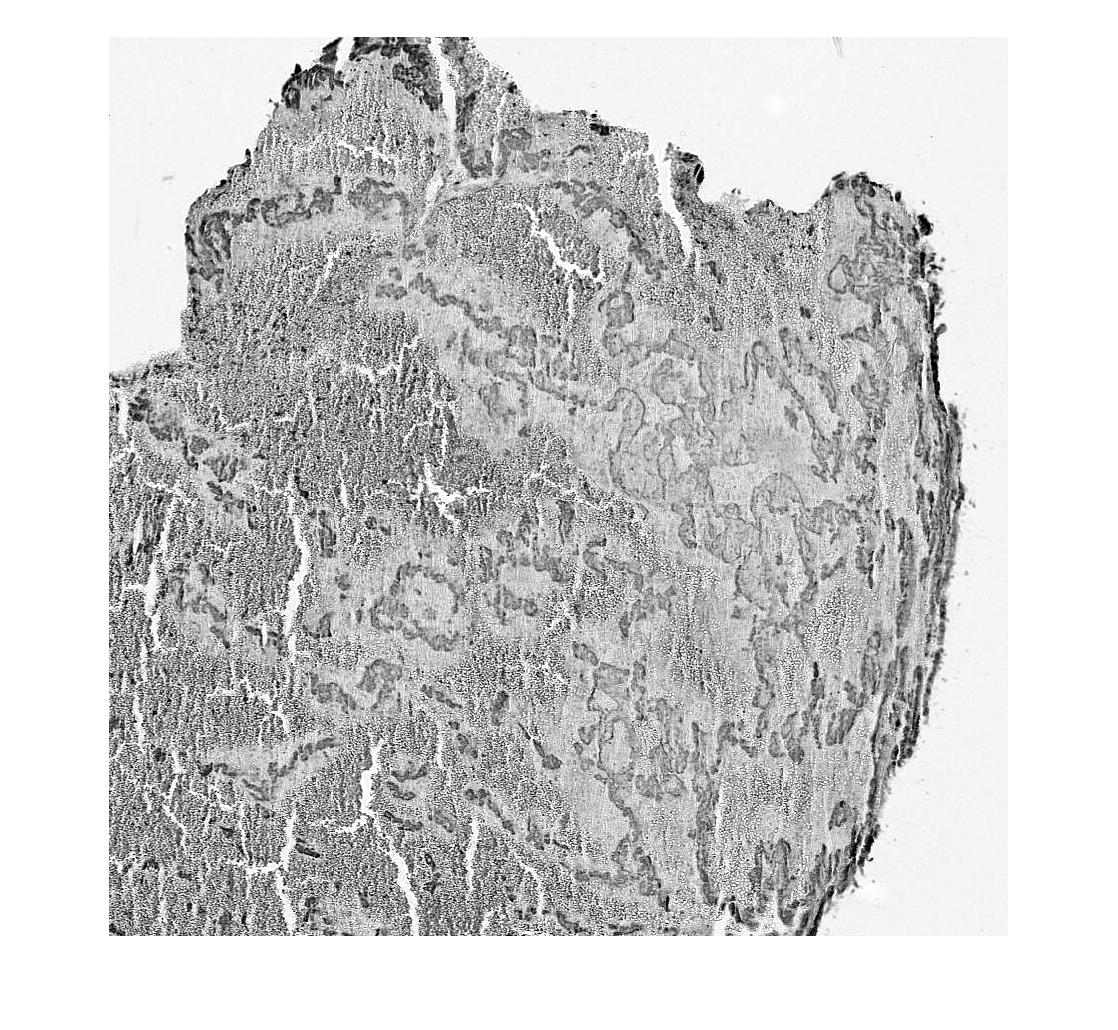
\includegraphics[width=4.5cm]{RGB_b}}}
	\caption{Illustratie van respectievelijk de rode, groene en blauwe kleurwaarden (\textit{RGB}). Hierbij komt wit overeen met de maximumwaarde en zwart met de minimumwaarde van die kleur.}
	\label{figuur RGB}
\end{figure}

\begin{figure}[H]
	\centering
	\subfloat[]{{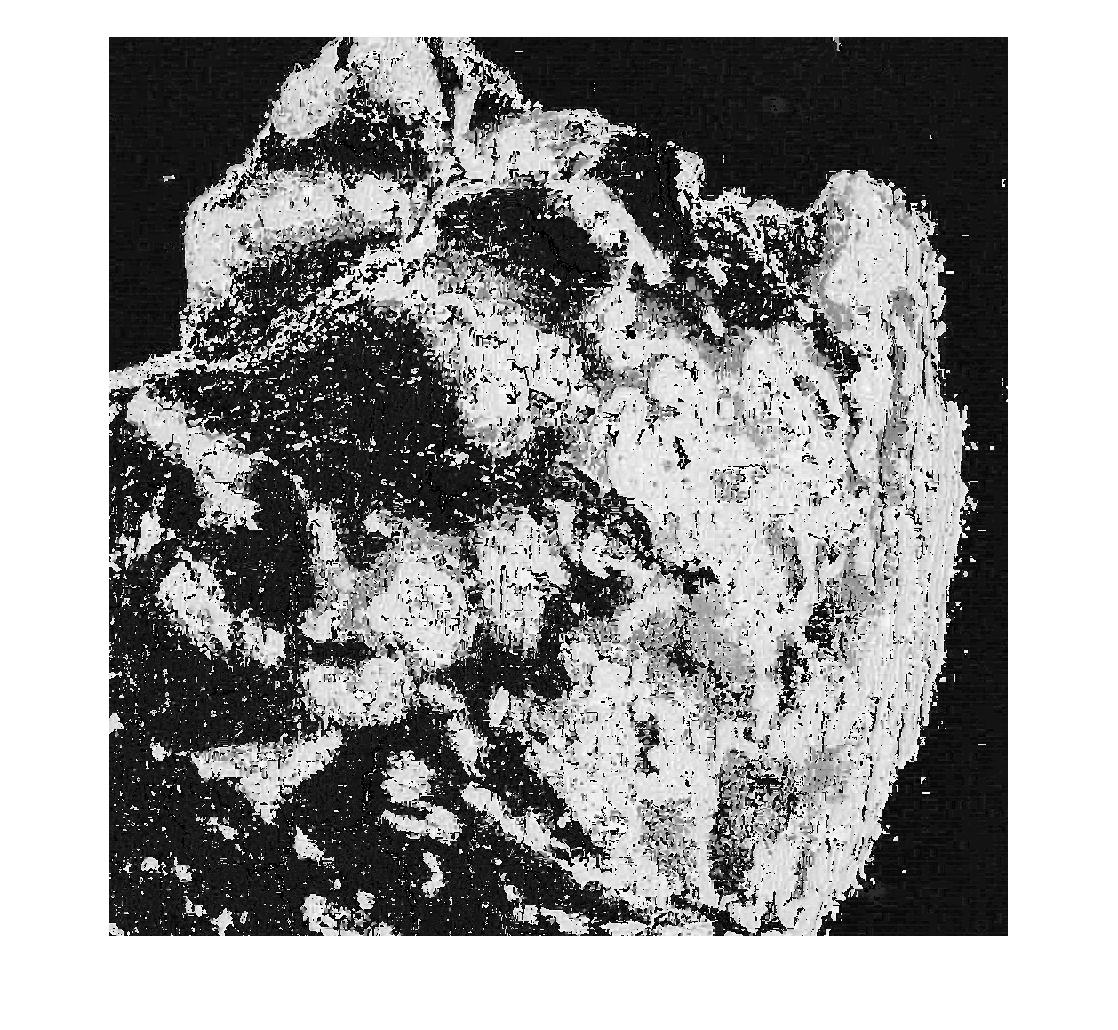
\includegraphics[width=4.5cm]{HSV_h}}}
	\qquad
	\subfloat[]{{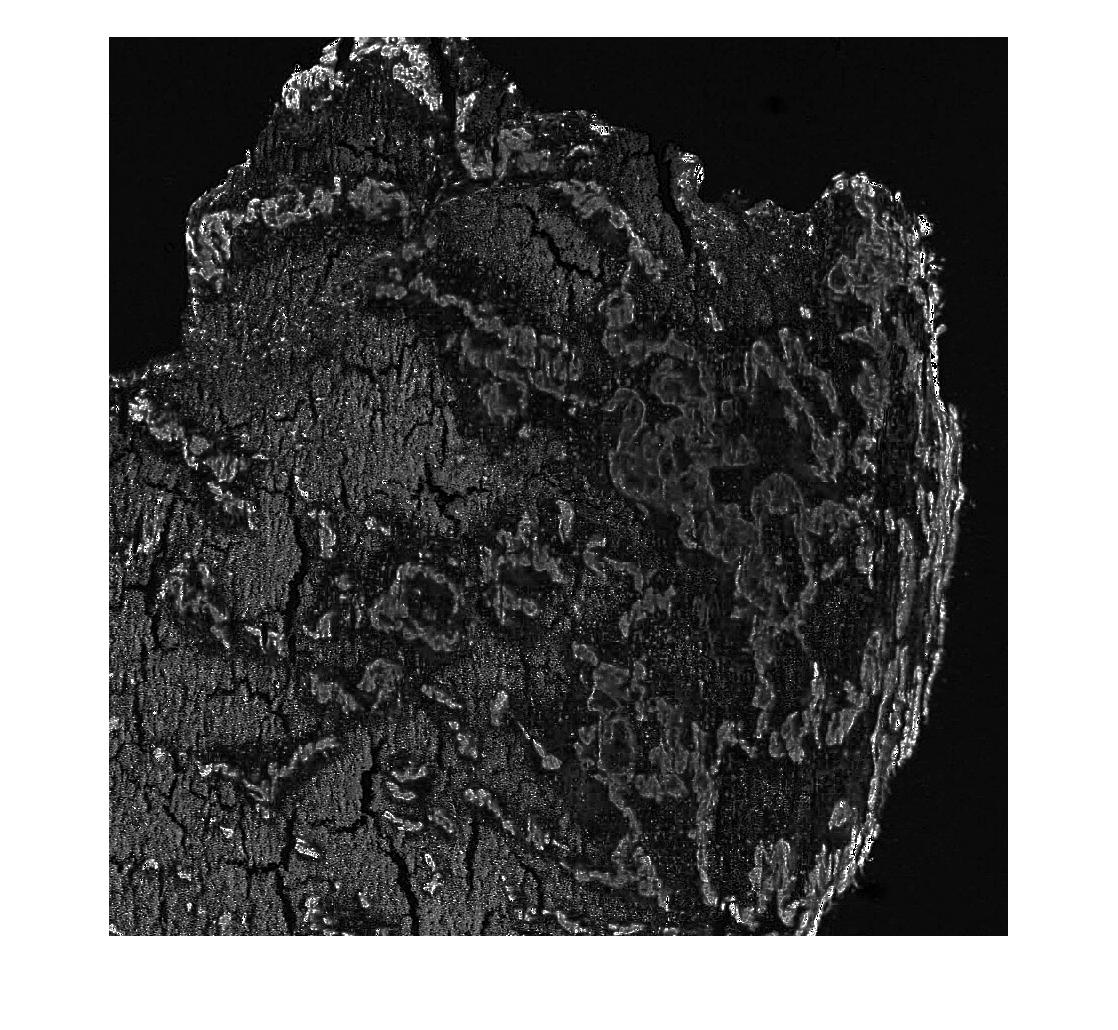
\includegraphics[width=4.5cm]{HSV_s}}}
	\qquad
	\subfloat[]{{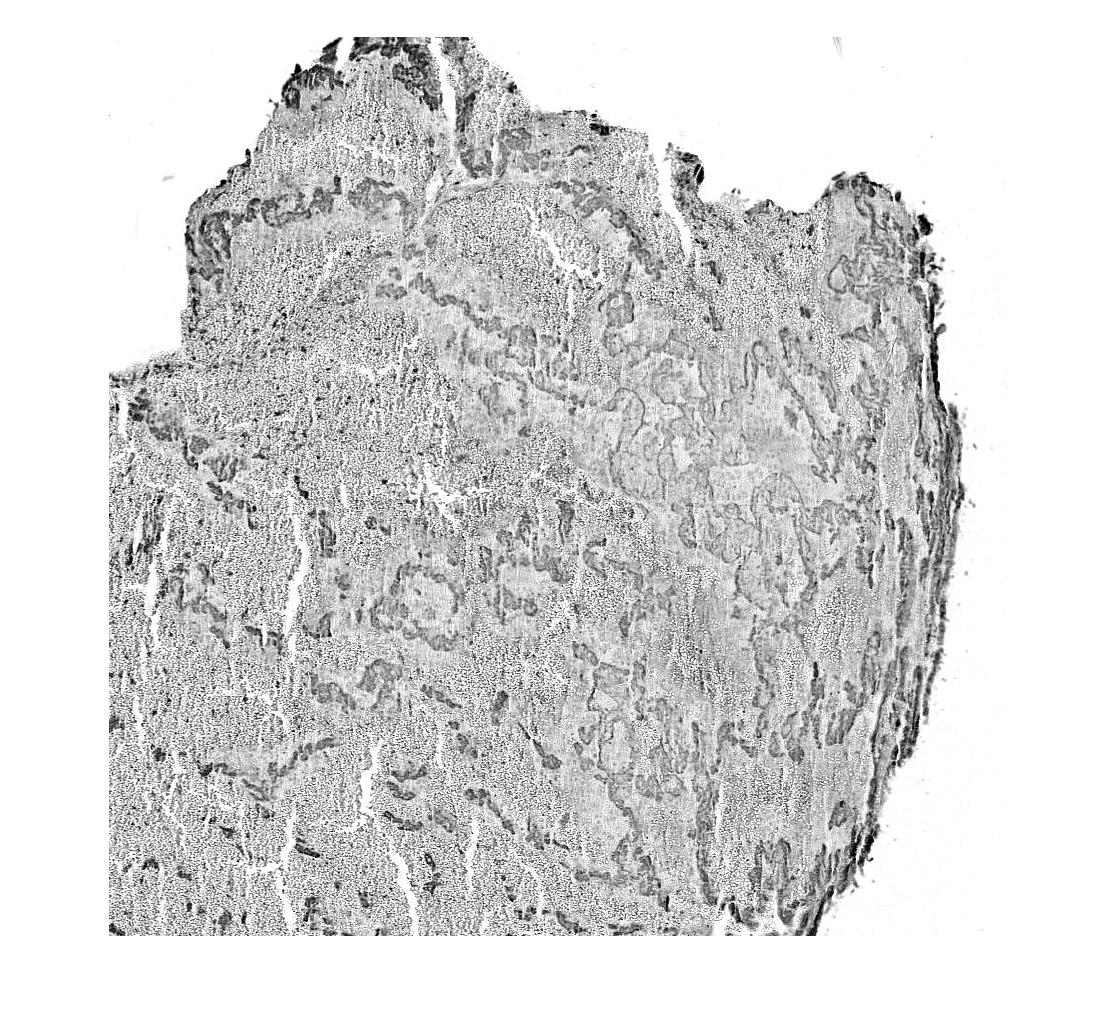
\includegraphics[width=4.5cm]{HSV_v}}}
	
	\caption{Illustratie van respectievelijk de \textit{hue}, \textit{saturation} en \textit{value} kleurwaarden (\textit{HSV}). Hierbij komt wit overeen met de maximumwaarde en zwart met de minimumwaarde van die kleurwaarde.}
	\label{figuur HSV}
\end{figure}

\subsubsection{Een algemene threshold}
De volgende stap is nu een filter bepalen voor alle indicatorpixels. Het probleem is echter dat een goede filter voor de ene foto niet altijd een goede filter voor de andere foto is. Daarom hebben we voor iedere foto manueel een 'threshold' bepaald en deze achteraf met elkaar vergeleken. Het resultaat is een vrij algemene threshold die alle indicatorpixels met zekerheid aanduidt. Af en toe worden jammer genoeg verkeerde pixels aangeduid. Het aantal is weliswaar niet zo groot, maar dit zullen we trachten te omzeilen in het volgende hoofdstuk. Een voorbeeld van deze algemene threshold is te zien op de Figuur \ref{figuur alg_tresh}.
\begin{figure}[H]
	\centering
	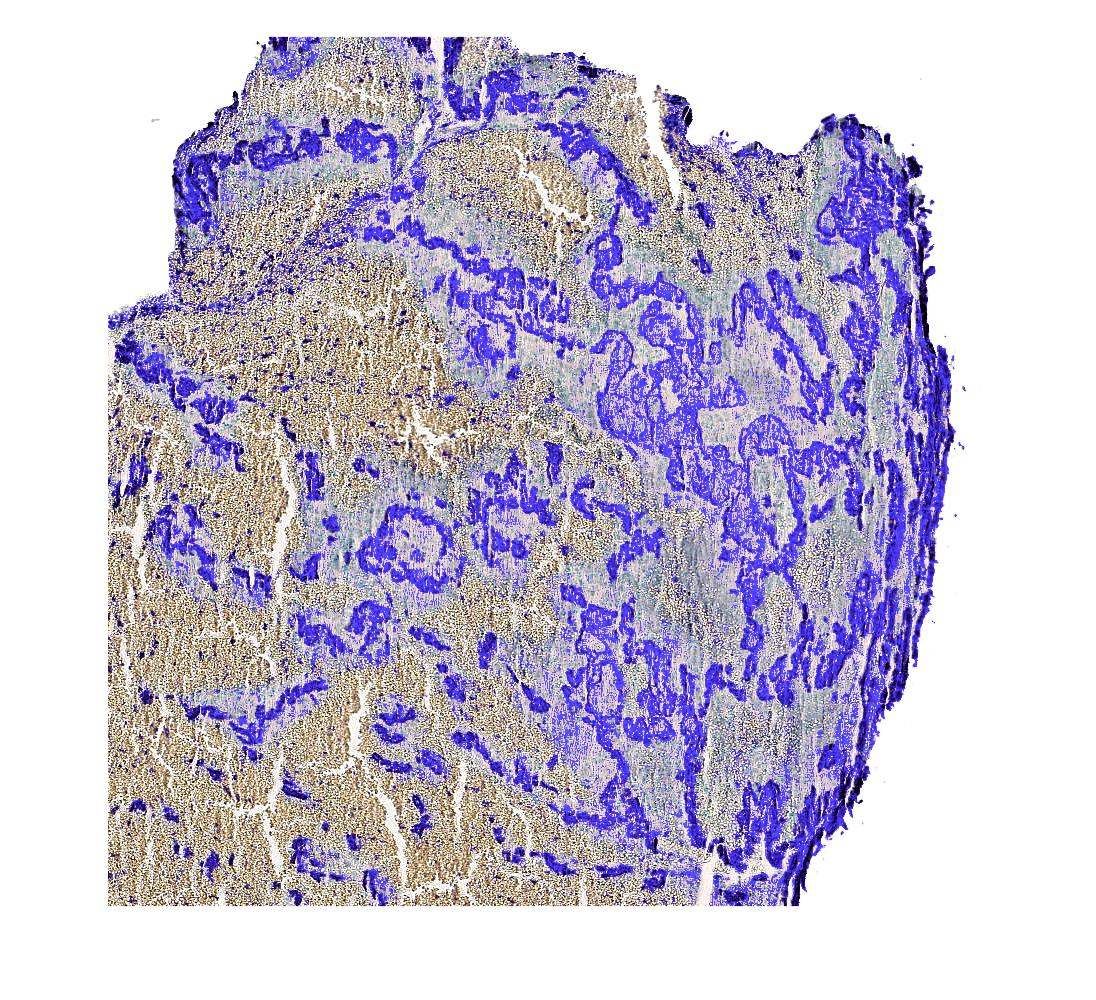
\includegraphics[width = 0.7\textwidth]{algemene_threshold}
	
	\caption{We hebben alle indicatoren met een blauwe kleur aangeduid. De algemene threshold selecteert alle indicatorpixels, maar jammer genoeg ook enkele verkeerde (voornamelijk rechtsonder).}
	\label{figuur alg_tresh}
\end{figure}

\subsubsection{Optimalisatie van de threshold}
In dit hoofdstuk willen we het aantal verkeerde pixels verminderen zonder de juiste te beïnvloeden. We hebben echter al een vrij goede threshold waardoor we een statistische analyse van wat onder deze mask ligt, kunnen uitvoeren. We stellen hiervoor een histogram van de \textit{HSV} kleurwaarden onder de mask op. Het levert ons namelijk een interessant resultaat dat te zien is in Figuur  \ref{figuur HSVHIST}. We zien namelijk duidelijke verschillen in de frequenties van de kleurwaarden. De grafieken tussen de verschillende afbeeldingen zijn nagenoeg gelijk van vorm, maar de pieken liggen soms meer dan 5\% verschoven.\\
Het idee is om nu de verkeerde pixels via deze diagrammen eruit te filteren. Indien we dat de verkeerde pixels essentieel in kleur verschillen van indicatorpixels en dat ze niet vaak voorkomen. Dan kunnen we in principe alle pixels met een frequentie onder een bepaalde grenswaarde schrappen. Een betere benadering is misschien om het punt te vinden, waar de frequentie van de pixels enorm begint toe te nemen of we met andere woorden grote 'indicatoraders' aan het verwijderen zijn. Dit punt kan theoretisch benaderd worden als het maximum van de tweede afgeleide naar de kleurwaarde. Hierdoor worden nog iets minder verkeerde pixels aangeduid zoals verwacht. Het nadeel is dat ook alle pixels met een waarde rond de 1 op Figuur  \ref{figuur HSVHIST} natuurlijk negeren. Waardoor deze weer manueel toegevoegd moeten worden.  
Een extra stap is tenslotte nog de indicatorpixels morfologisch te sluiten met een algoritme dat reeds in MATLAB verwerkt is. Dit is zeer nuttig omdat de indicatorpixels meestal met elkaar verbonden zijn en daardoor deze weer onderling kunnen verbinden.


\begin{figure}[H]
	\centering
	\subfloat[]{{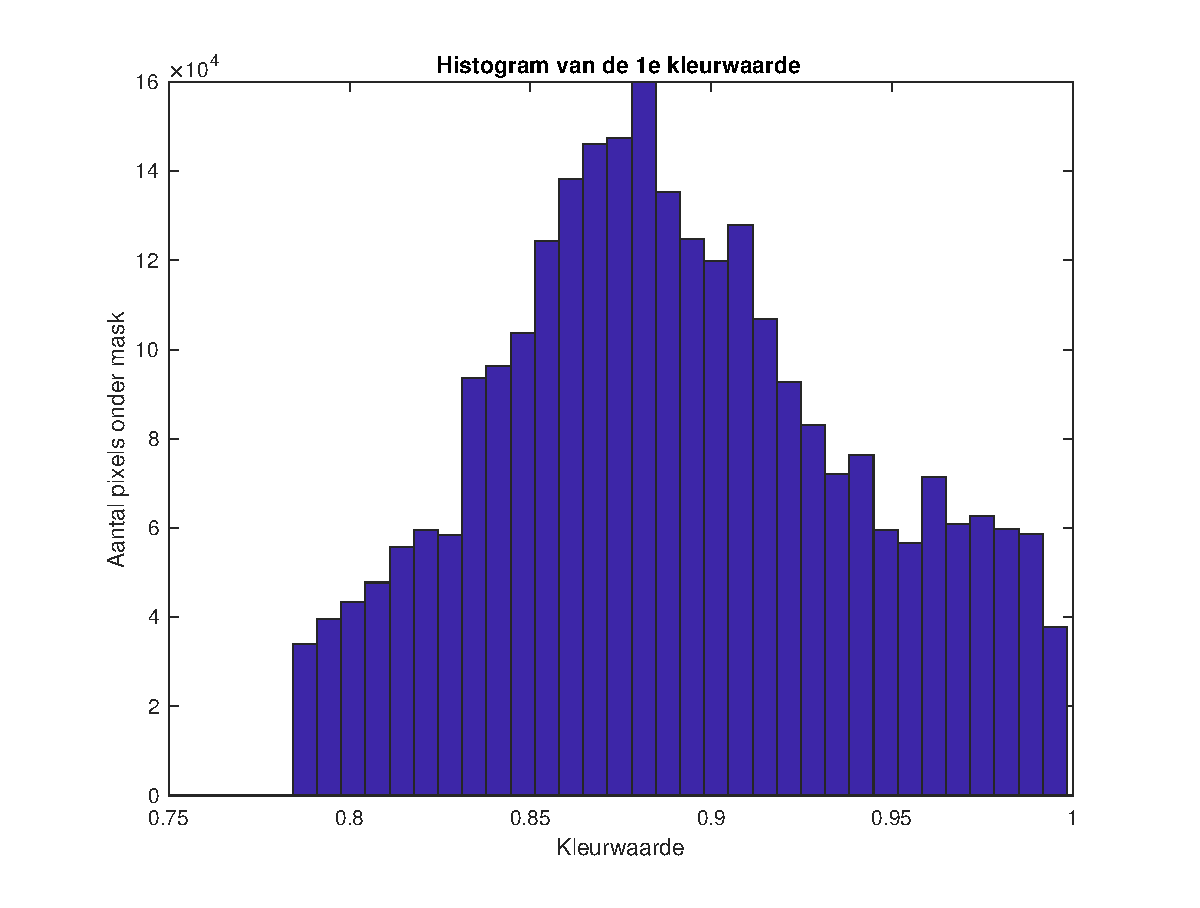
\includegraphics[width=4.5cm]{hsvhist_h}}}
	\qquad
	\subfloat[]{{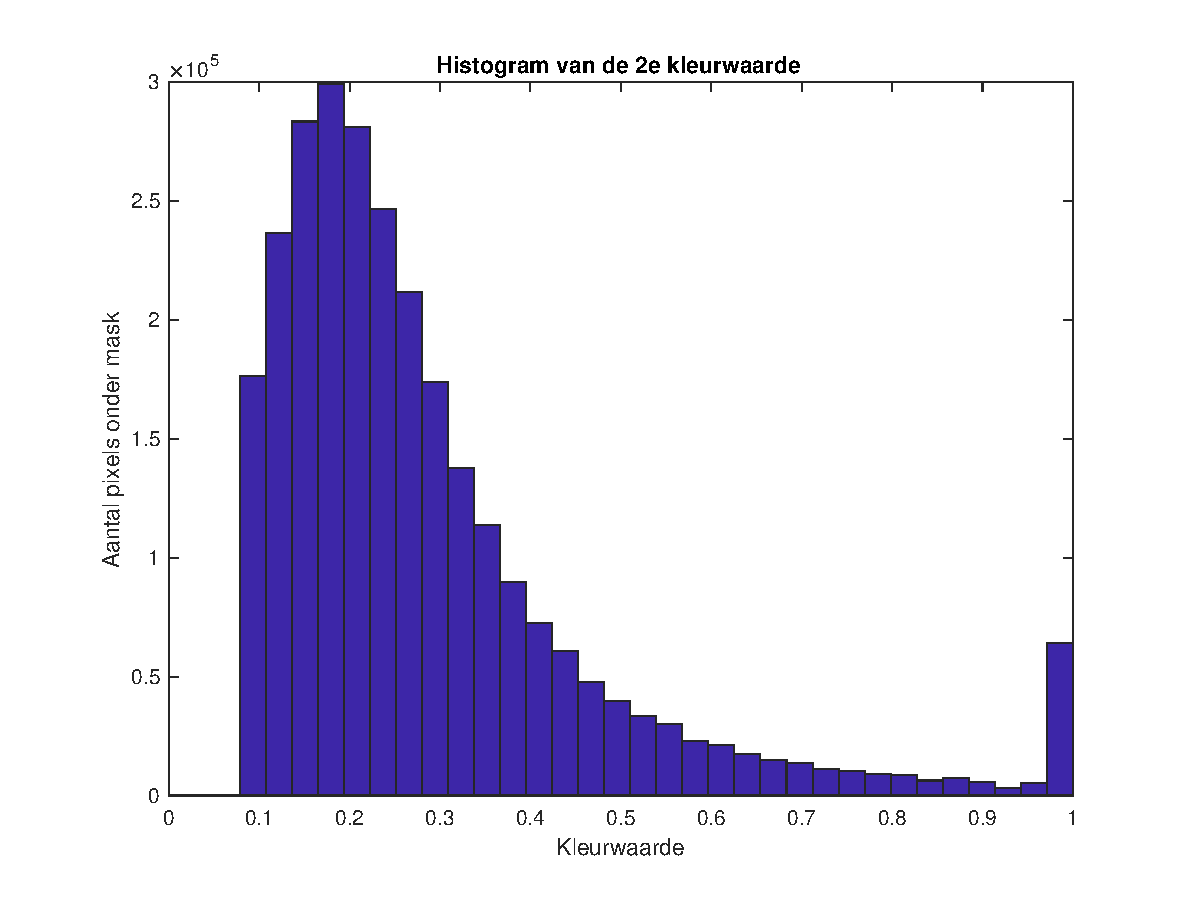
\includegraphics[width=4.5cm]{hsvhist_s}}}
	\qquad
	\subfloat[]{{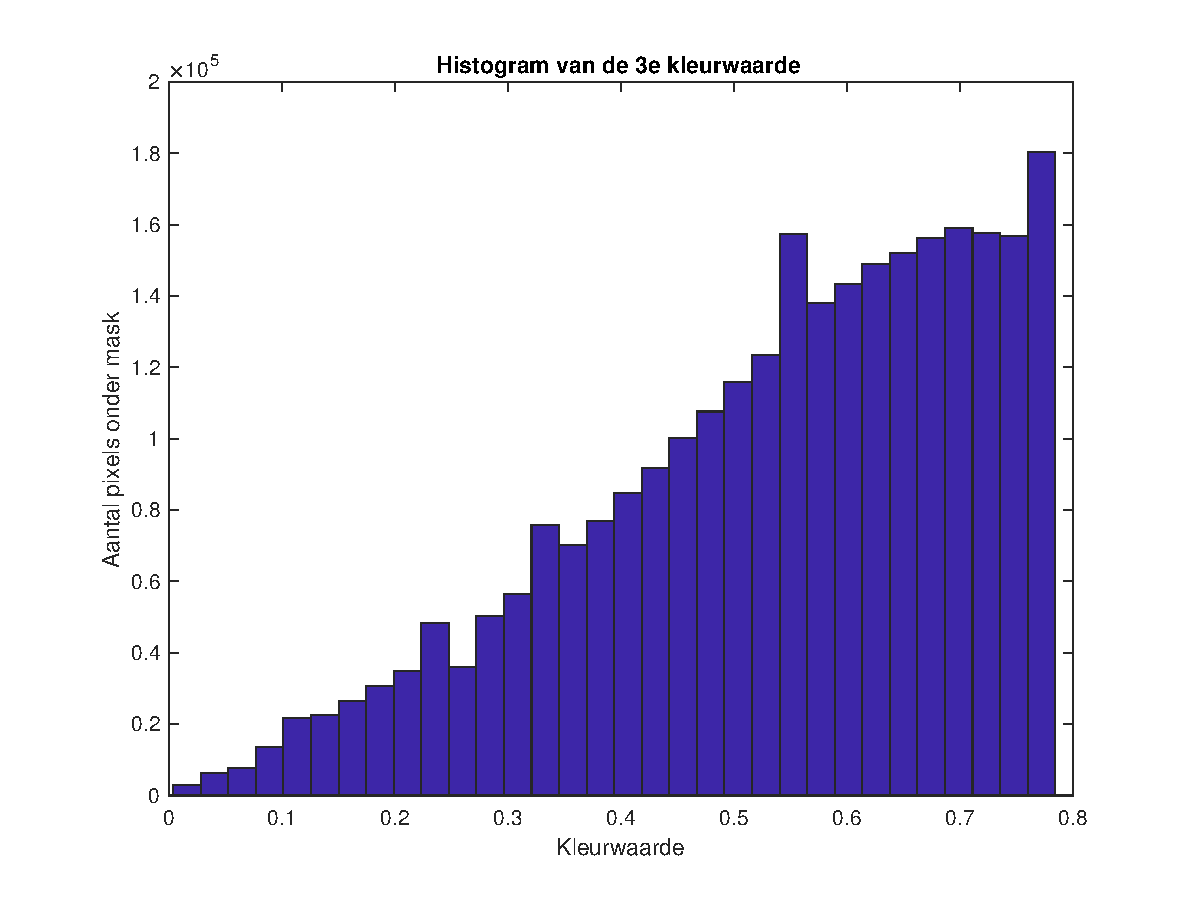
\includegraphics[width=4.5cm]{hsvhist_v}}}
	
	\caption{Histogrammen van de HSV kleurwaarden. We zien duidelijk het verschil in frequenties.}
	\label{figuur HSVHIST}
\end{figure}

\begin{figure}[H]
	\centering
	\subfloat[]{{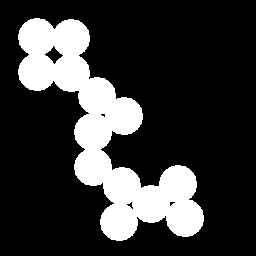
\includegraphics[width=7cm]{morf_open}}}
	\qquad
	\subfloat[]{{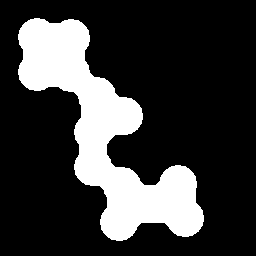
\includegraphics[width=7cm]{morf_gesloten}}}
	
	\caption{Illustratie waarbij de witte cirkels uit afbeelding (a) morfologisch gesloten worden in afbeelding (b)}
	\label{figuur morf}
\end{figure}
	
	
	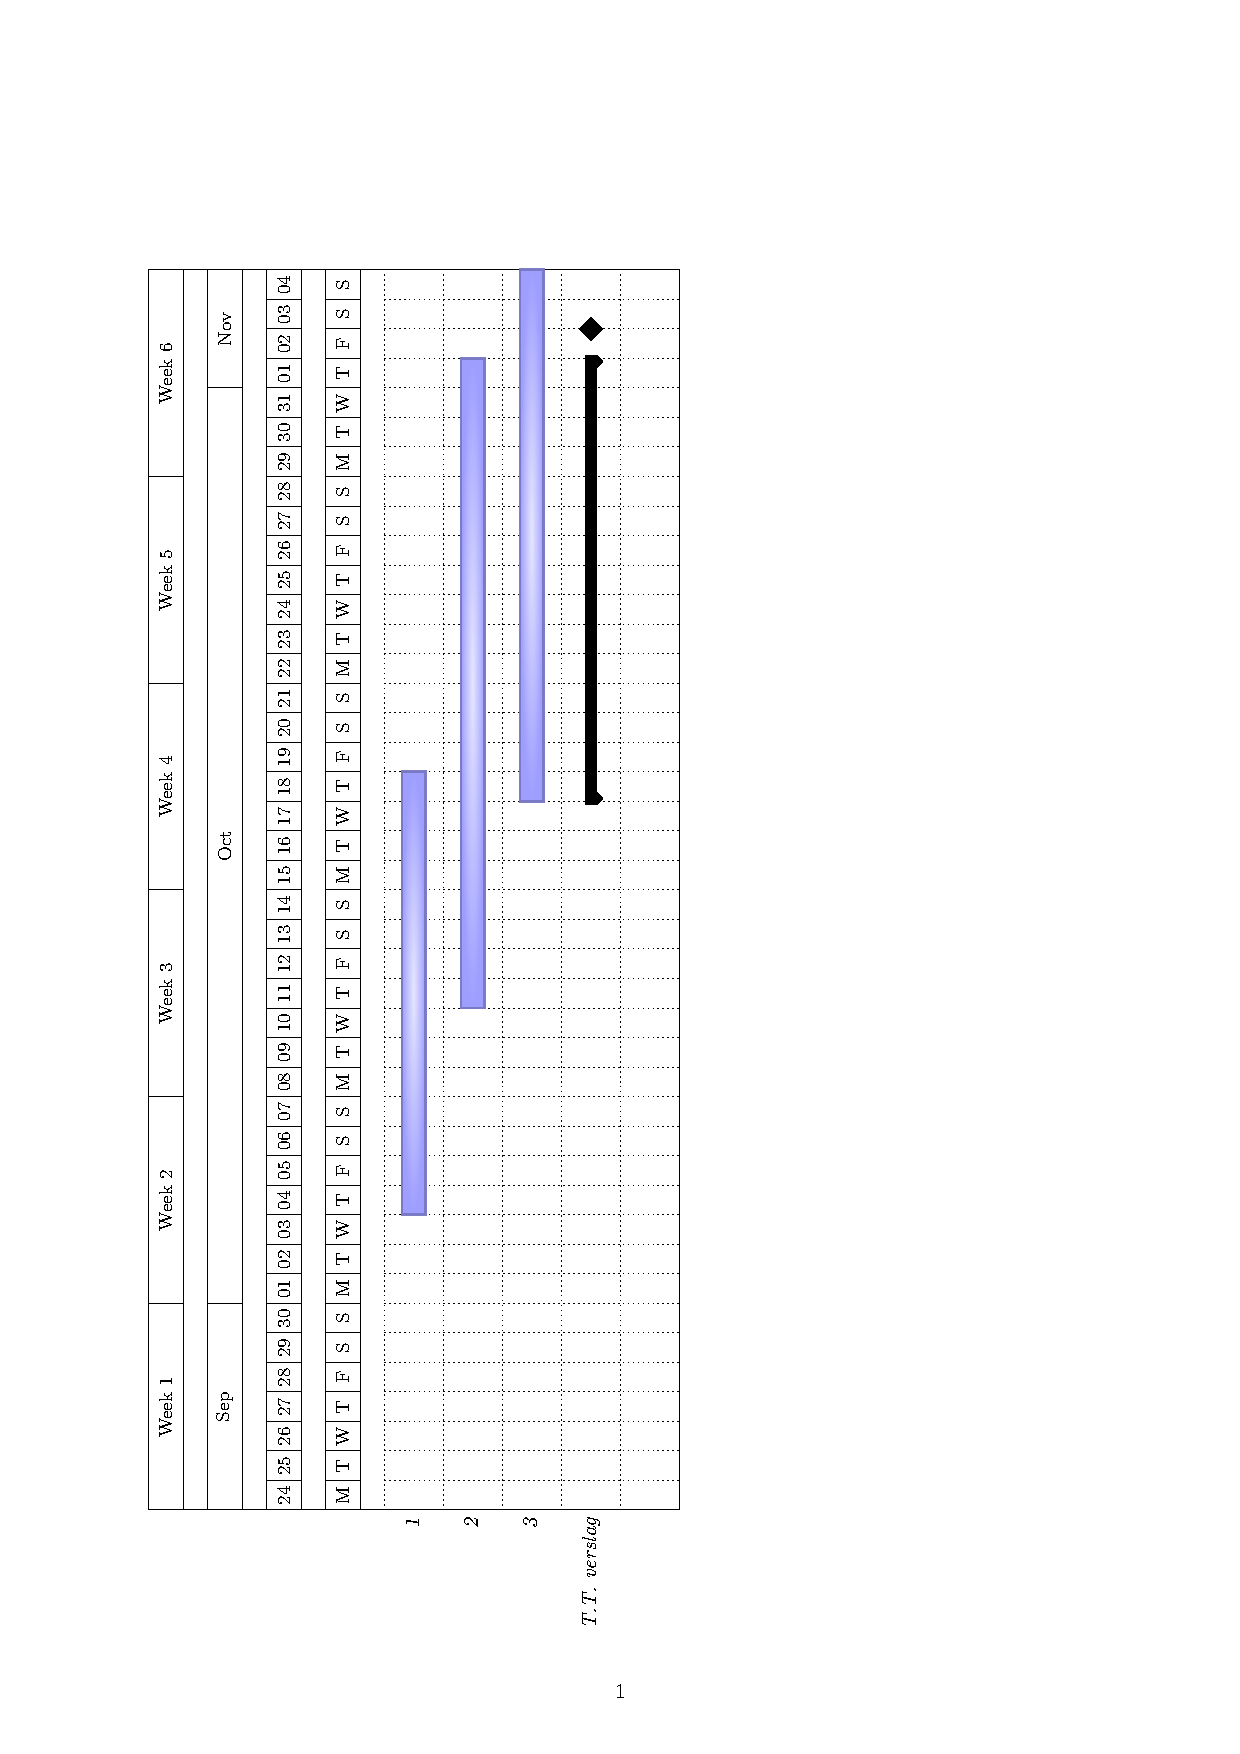
\includepdf[page={1-3}]{ganttchart}	
	
	

\end{document}
